\documentclass[10pt, a4paper]{article}

% Text packages
\usepackage[french]{babel}
\usepackage[utf8]{inputenc}
\usepackage{lmodern} % Latin founts

% Fonts packages
\usepackage{ifxetex}
\ifxetex
    \usepackage{fontspec}
    \setmainfont{OpenDyslexic}
\else
    \usepackage[T1]{fontenc}
\fi

% Math fonts
\usepackage{amsmath}
\usepackage{amsfonts}
\usepackage{latexsym}

% Theorem fonts
\usepackage{amsthm}

% Title import
\usepackage{authoraftertitle}

% Clickable link
\usepackage{hyperref}
\hypersetup{
    colorlinks=true,
    citecolor=blue,
    filecolor=black,
    linkcolor=black,
    urlcolor=blue
}

% Image side by side
\usepackage{subcaption}

% Text color
\usepackage{xcolor}

\usepackage{xspace}

% Image
\usepackage{graphicx}
\graphicspath{ {./images/} }
\usepackage{bookmark}

% Code import
\usepackage{minted}
\usemintedstyle{emacs} % borland

\title{PaP}
\author{BERASATEGUY Tanguy, GOEDEFROIT Charles}

\begin{document}

% Front page
\vspace*{\stretch{1}}
\begin{center}
    \textbf{\LARGE\MyTitle}
    \\[.5cm]
    \textbf{Projet : rapport2}
    \\[.5cm]
    4TIN804U
    \\[.5cm]
    \MyAuthor
\end{center}
\vspace*{\stretch{1}}

\newpage

\tableofcontents

\newpage

\section{ILP optimization (4.1)}

On as fait les modifications :

Pour \emph{ssandPile\_do\_tile\_opt()} on a retirer les appelles à \em{table(out, i, j)}
pour passer par une varaible intermedier result. Cette modification petmer au compilateur
de vectoriser car il peut maintenet facilement voir que les différante lige peuve être 
calculer en paralelle.\\

Nouas avons modifier c'est lignes :
\inputminted[
    frame=lines,
    framesep=2mm,
    baselinestretch=1.2,
    fontsize=\footnotesize,
    linenos,
    firstline=1,
    lastline=25
]{diff}{codes/sync_do_tile_opt.c}

Le code de la fonction final :
\inputminted[
    frame=lines,
    framesep=2mm,
    baselinestretch=1.2,
    fontsize=\footnotesize,
    linenos,
    firstline=27,
    lastline=45
]{c}{codes/sync_do_tile_opt.c}

Nous avons verifier et on obtient le même résultats et le même nombre d'iterations (69190)
avec la version par défaut et la version opt.\\
\begin{figure}[H]
    \centering
    \begin{subfigure}{.4\textwidth}
        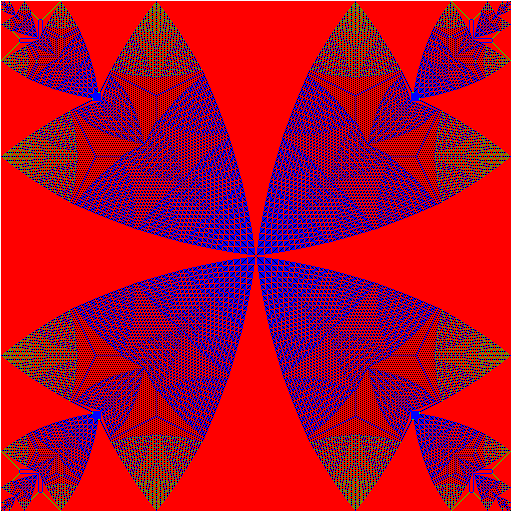
\includegraphics[width=1\linewidth]{dump-ssandPile-seq-dim-512-iter-69190_default}
        \caption{\small{avec do\_tile\_default}}
        \label{fig:ssandPile_default}
    \end{subfigure}
    \begin{subfigure}{.4\textwidth}
        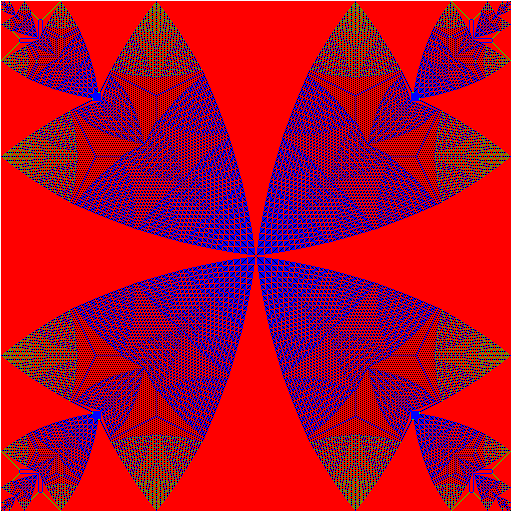
\includegraphics[width=1\linewidth]{dump-ssandPile-seq-dim-512-iter-69190_opt}
        \caption{\small{avec do\_tile\_opt}}
        \label{fig:ssandPile_opt}
    \end{subfigure}
    \caption{Verification du résultats pour ssandPile}
\end{figure}

Le gain de performance est de $2.37$ car $\frac{178812}{75408}$
\\[0.5cm]

Pour \em{asandPile\_do\_tile\_opt()} on a retirer...

Nouas avons modifier c'est lignes :
\inputminted[
    frame=lines,
    framesep=2mm,
    baselinestretch=1.2,
    fontsize=\footnotesize,
    linenos,
    firstline=1,
    lastline=24
]{diff}{codes/async_do_tile_opt.c}

Le code de la fonction final :
\inputminted[
    frame=lines,
    framesep=2mm,
    baselinestretch=1.2,
    fontsize=\footnotesize,
    linenos,
    firstline=26,
    lastline=46
]{c}{codes/async_do_tile_opt.c}

Nous avons verifier et on obtient le même résultats et le même nombre d'iterations (34938)
avec la version par défaut et la version opt.\\
\begin{figure}[H]
    \centering
    \begin{subfigure}{.4\textwidth}
        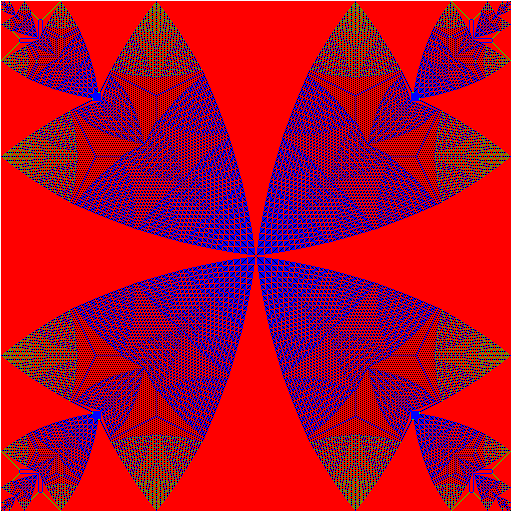
\includegraphics[width=1\linewidth]{dump-asandPile-seq-dim-512-iter-34938_default}
        \caption{\small{avec do\_tile\_default}}
        \label{fig:asandPile_default}
    \end{subfigure}
    \begin{subfigure}{.4\textwidth}
        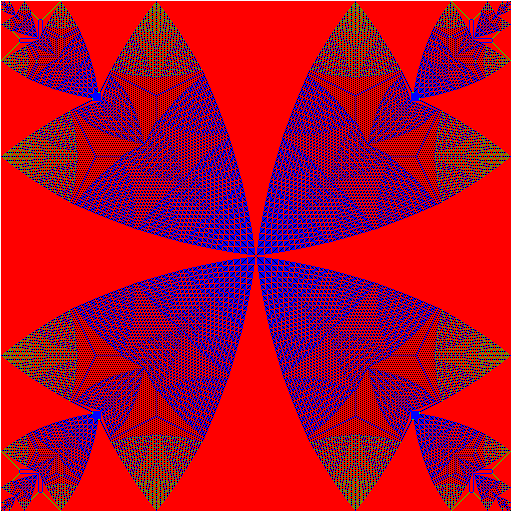
\includegraphics[width=1\linewidth]{dump-asandPile-seq-dim-512-iter-34938_opt}
        \caption{\small{avec do\_tile\_opt}}
        \label{fig:asandPile_opt}
    \end{subfigure}
    \caption{Verification du résultats pour asandPile}
\end{figure}

Le gain de performance est de $1.2$ car $\frac{37990}{31405}$

\section{OpenMP implementation of the synchronous version (4.2)}

\begin{figure}[h]
    \centering
    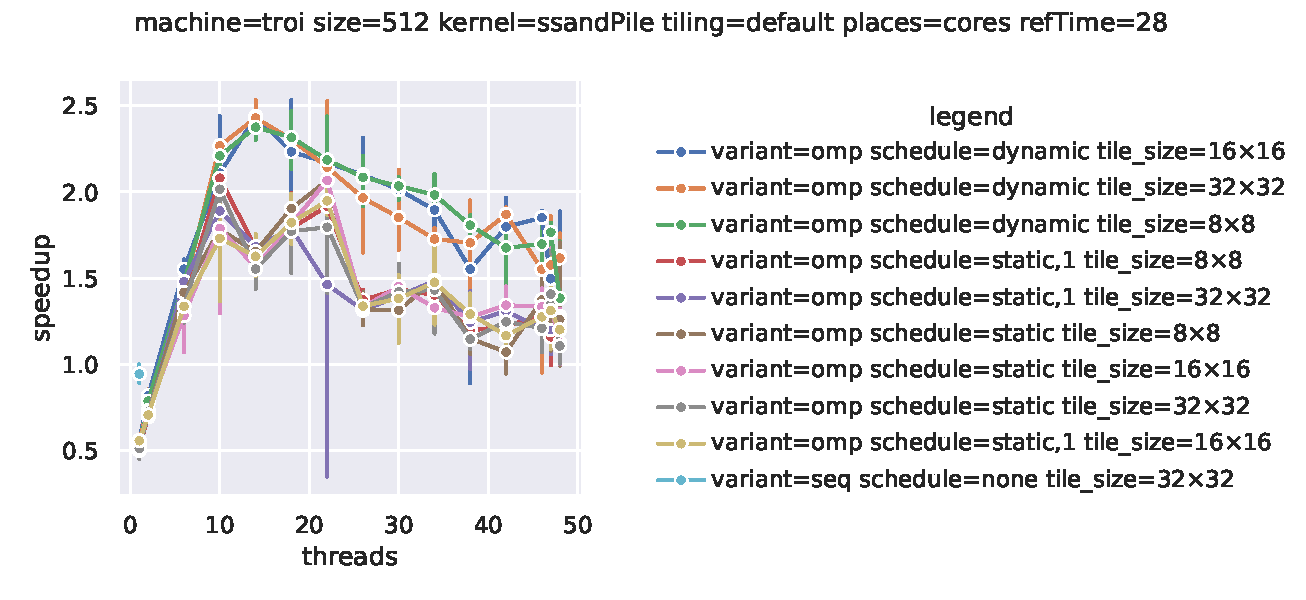
\includegraphics[width=1\linewidth]{ssand_omp.pdf}
\end{figure}

\begin{figure}[H]
    \centering
    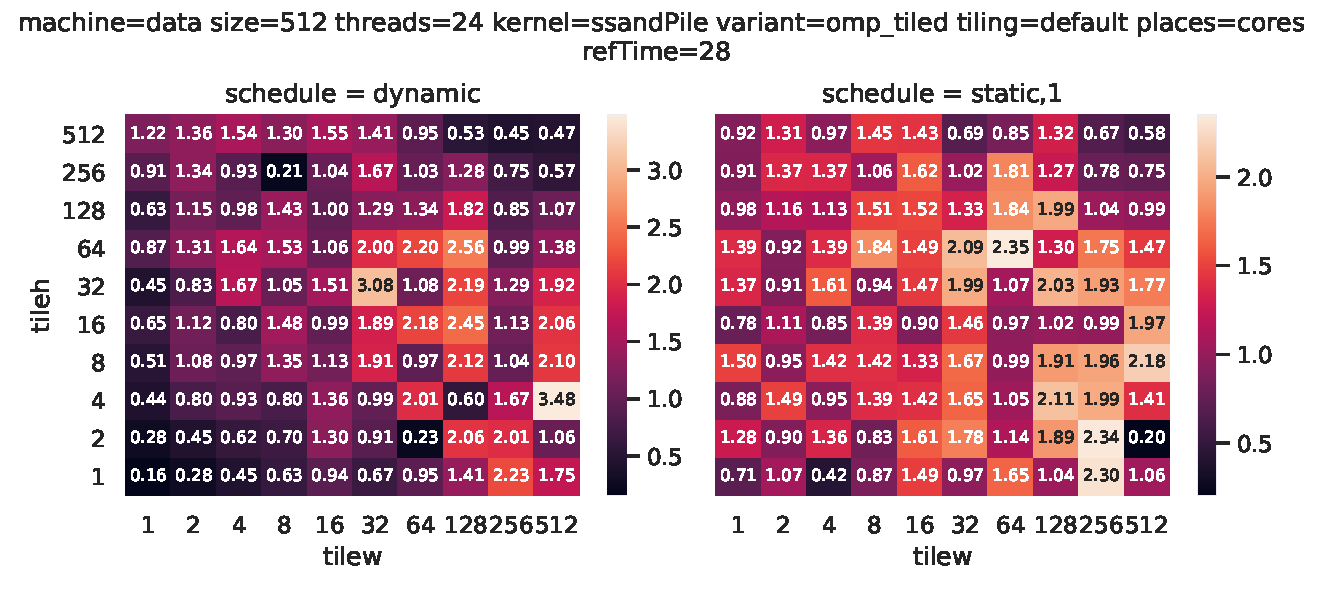
\includegraphics[width=1\linewidth]{ssand_omp_tiled.pdf}
\end{figure}

\section{OpenMP implementation of the asynchronous version (4.3)}

\section{Lazy OpenMP implementations (4.4)}



% \begin{listing}[!ht]
%     \inputminted[
%         frame=lines,
%         framesep=2mm,
%         baselinestretch=1.2,
%         fontsize=\footnotesize,
%         linenos
%     ]{c}{codes/test.c}
%     \caption{Example from external file}
%     \label{listing:1}
% \end{listing}

% \includegraphics[height=1.5cm]{<image>}

\end{document}